\documentclass[12pt, titlepage]{article}

\usepackage{float}
\usepackage{booktabs}
\usepackage{tabularx}
\usepackage{hyperref}
\usepackage{graphicx}
\usepackage{titling}
\usepackage[utf8]{inputenc}
\usepackage{graphicx}
\usepackage{gensymb}
\usepackage{siunitx}
\usepackage{textcomp}
\usepackage{longtable}
\graphicspath{{./images/}}
\usepackage{array}
\graphicspath{ {figures/} }

\hypersetup{
    colorlinks,
    citecolor=black,
    filecolor=black,
    linkcolor=blue,
    urlcolor=blue
}
\usepackage[round]{natbib}
\begin{document}

\title{
    MobiCharged\\Design Document 
    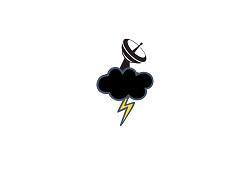
\includegraphics[width=9cm]{images/mobicharged.png} 
}
\author{Team Super Charged (No.33)
		\\ Nashit Mohammad - mohamn31
		\\ Eric Nguyen - nguyee13
		\\ Samuel De Haan - dehaas1
		\\ Eamon Earl - earle2
		\\ Mustafa Choueib - choueibm
}
    

\date{January 18th, 2023}


\maketitle

\pagenumbering{roman}
\tableofcontents
\listoffigures
\listoftables

\vspace{20pt}
\begin{center}
\begin{table}[H]
\caption{\bf Revision History}
    \begin{tabular}{p{2cm}p{3cm}p{2cm}p{6cm}}
    \hline
    \bf Author & \bf Date & \bf Version & \bf Description\\
    \hline
    All & January, 2023 & Rev 0 & Created first draft of document\\
    \hline
    \end{tabular}
\end{table}
\end{center}

\newpage

\pagenumbering{arabic}

\section{System Overview}

\subsection{Naming Conventions and Terminology}

\begin{table}[htp]
\caption{\bf Naming Conventions and Terminology}
\begin{tabular}{ |p{6cm}|p{8cm}|  } 
 \hline
\bf Word/Acronym & \bf Definition/Context\\
 \hline
 Functional Requirement & Requirements that describe what the product is supposed to do\\
 \hline
Non-functional Requirement & Requirements that describe qualities that product will have\\
 \hline
General Contractor & Third party companies that acquire services by Mobilite-Power\\
 \hline
Data Smoothing & The process of using old data as well as "future" data in order to predict designs\\
 \hline
ML & "Machine Learning" algorithm\\
\hline
AC & Ancticipated Change\\
\hline 
R & Requirement\\
\hline 
UC & Unlikely Change\\
\hline 
A & Assumption\\
\hline 
DS & Download Speed\\
\hline
US & Upload Speed\\
\hline
\end{tabular}
\end{table}

\subsection{Relevant Facts and Assumptions}
\begin{itemize}
    \item There is an assumption that the developers will eventually have access to enough processing power to conduct large quantities of simulations.

\end{itemize}

\subsection{Introduction}

Engineers are tasked with design in construction to exceed requirements without hindering safety. Safety is a topic that is never missed within the industry and is continuously being highlighted amongst designs; especially as Engineers are reminded of their moral obligations to society by their awarded rings upon graduation. 
\par
As a current process, the construction industry places sensors within concrete spaces to continuously test and/or monitor the integrity of buildings during as well as after construction. Ultimately however, these sensors run out of battery and are required to be re-charged.
\par
The industry still faces challenges when attempting to charge these sensors with the method of remote charging as the current products that satisfy remote charging abilities are yet to be optimized. There are a significant number of buildings being built in the GreaterToronto-Area, which is emphasized considering that 70\% of cranes within Canada are in just the GTA alone. To place innovation in the sub-field of safety within the industry, it is indeed a requirement to modernize the ability of producing efficient remote charging systems and to have the design process optimized to provide the most effective results.
\par
The system-solution for this will be the development of MobiCharged. 


\subsection{Purpose}

\subsubsection{System Purpose}
The purpose of the development of MobiCharged is to assist stakeholders in the infrastructure development industry revolving around design and construction which include but are not limited to; consultant engineers, contractors and building owners. 
\par
The software will aid remote charging designers by optimizing their design through the method of machine learning, which will substantially reduce their time \& efforts designing as it will remove the process of costly simulations. 
\par
The hardware will serve as a prototype and be used for demonstration purposes for the aid in display as well as understanding of limitations for the software. 

\subsubsection{Document Purpose}
The purpose of this document is to elucidate the decomposition of the system (both the software portion as well as the hardware) into its components and provide a modular understanding for each component in the system. This document will serve as a guide for the execution of production intended to be completed in the upcoming weeks.


\section{Scope}
\subsection{System Summary}
The environments in which these physical systems operate are typically from roof-tops and/or high-altitude locations with spacial capabilities to place arrays of these systems. These systems react to user inputted (remotely) data such as the location of the device required to be charged, so that it may orient itself in a manner optimal for that application. 
\par
The purpose of the software system, MobiCharge, is a machine learning algorithm that will be used by Mobilite-Power, engineering consultant groups, general contractors and building maintenance teams to optimize the design process required to effectively and efficiently produce the most viable remote charging system. In doing so, this will negate the current process of manually conducting simulations (that requires lengthy computerized numerical calculations), ultimately minimizing cost, manual labor, and the time necessary to produce the required results. This system will provide users with the optimal configuration of a remote charging device based on the desired output, encrypt data protecting users when producing design results and use data smoothing to ensure the accuracy of the system in a time efficient manner.
\par
The hardware system is to root our algorithms optimization in the real world environment. The production of a physical model will assist in the determination of the absolute boundaries that can be fed into the machine learning algorithm. Variable parameter ranges will be able to be derived from the physical model to determine the magnitude to which the boundaries can be pushed within the simulation. The physical system provides a secondary purpose in the form of data collection and verification. In order to increase the breadth of data that we can feed into the algorithm, we must determine the degree of computational error within the simulation results. A physical model will aid in determining this range and lead to further optimization through the machine learning algorithm.

\subsection{Assumptions}
\textbf{A1:} Developers will have access to enough processing power to conduct large quantities of simulations
\par
\textbf{A2:} User does not intentionally attempt to enter inputs incorrectly, as well as provide positive feedback to the system when it is not correct
\par
\textbf{A3:} Users have access to wifi with sufficient speeds, averaging 15 Mbps DS \& 10 Mbps US
\par
\textbf{A4:} Users execute the software with Windows 10 OS (or higher) as instructed
\par 
\textbf{A5:} The average developer has background knowledge in electromagnetic theory
\par 
\textbf{A6:} The app will be used by the above-average tech savvy individual due to the niche in industry
\par
\textbf{A7:} Hardware will have sufficient power sources (specific current values are to be determined)
\par
\textbf{A8:} Weather conditions for the hardware are not extreme, i.e. not operating in storm conditions or temperatures below -35C or above 35C
\par
\textbf{A9:} Hardware is not used near other equipment which can create wave interferences 
\par 
\textbf{A10:} Hardware is to not be operated near magnetic materials
\par
\textbf{A11:} Users can be individually identifiable through email addresses and/or usernames (to be determined)

\section{Project Overview}
\subsection{Normal Operation}
This application is to be used by Mobilite-Power to reduce overhead costs associated with developing remote charging devices. The company will be able to use this system on their computers with ease.By using this system, Mobilite-Power will be able to minimize the cost, time, and labor required to determine the optimal configuration necessary for remote charging devices. This will make their operations more efficient.
\subsection{Behaviour Overview}
This system will continuously learn and develop without an operator. However, the ultimate output of the system will be event based, thus, requiring the user to initiate operations. The user will be required to provide the necessary input, in which the machine learning algorithm will return the optimal configuration for a remote charging device, encrypt the provided output, and store the optimal data into a database for data smoothing. When the system is not in use, it will be running simulations automatically to continuously refine its ability to produce accurate optimal results.
\subsection{Undesired Event Handling}
Undesired event handling is critical to ensuring that, even in unintended circumstances, the system can safely revert to a desired state. Thus, the system should ensure that in the event of an error or fault, it has a failsafe state to transition to. This fail-safe state will ensure that there are no corruptions in data, the system itself, or extensive damages caused. 

\section{System Contexts}

\subsection{Preliminary System Contexts}
The system will interact with pre-existing matlab simulation programs, purely at the simulations’ start and end points, where the program will pull data from completed simulations and push parameters to run new ones. In the early stages of the product life cycle, it will mainly be pulling the completed simulation data, and feeding it into the deep learning algorithm in order to train it and give it some experience with optimal solutions. This will require integration with large databases in order to record this data. 
\par
Once the core program / deep learning algorithm has been trained to some satisfying degree, the context will expand to include the second half of the cyclical integration with the pre-existing simulation software; it will now take charge of running new simulations that push the boundaries of its current knowledge base. This is in order to take full advantage of free processing power, such that the simulations are always being run, and the deep learner is constantly being trained. This may require interfacing with an additional software module in order to schedule data coming in to be processed, and outward data to be procured.
\par 
Later in the life cycle of the program, we will be either integrating with Mobilite’s current remote desktop server (used to run the simulations remotely), or develop our own, and the specifics of this contextual decision will depend on the availability of their server at this time. The goal would be to integrate our program with the server such that our deep learner would be able to access the data from any simulation run, and not just those on the local devices of our teams, which also implies that we plan on having these simulations able to be run on multiple different devices at the same time, eventually adding further scheduling and concurrency constraints to our learner-server pair. 
\par
Evidently, our context shifts and expands multiple times throughout the development lifecycle, as we wish to integrate with and expand upon pre existing software in multiple areas of the design. The following context diagrams give an idea of this development, with each diagram associated, in order, with the above paragraphs. The components will be briefly described alongside each diagram for clarity.

\begin{figure}[htp]
    \centering
    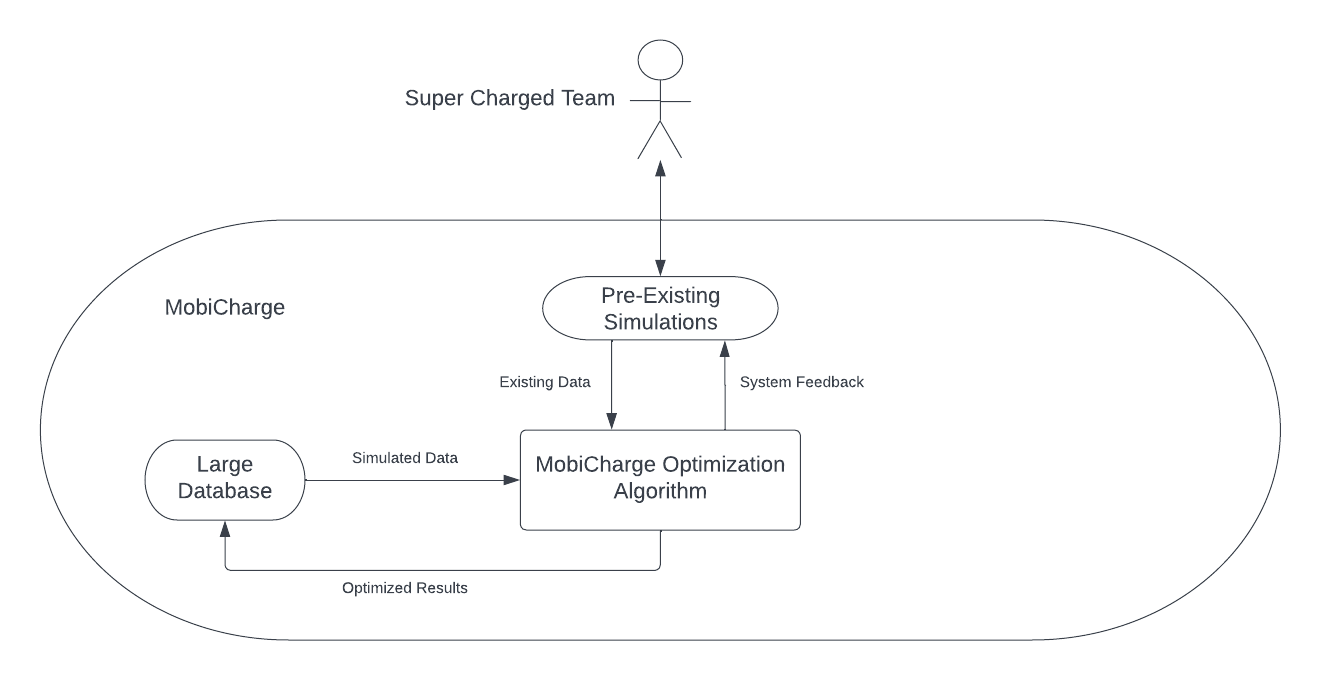
\includegraphics[width=15cm]{images/context0.png}
    \caption[Prelim System Contexts 1]{First stage of preliminary system context.}
    \label{fig:figure1}
\end{figure}

The external entity, the Super Charged team; the team of developers for the system, will begin to train the MobiCharged software system using pre existing simulation data. The simulations that are optimized by the system will then be stored into a large database for further use by the system. As shown by figure 1. \par
\newpage
\begin{figure}[htp]
    \centering
    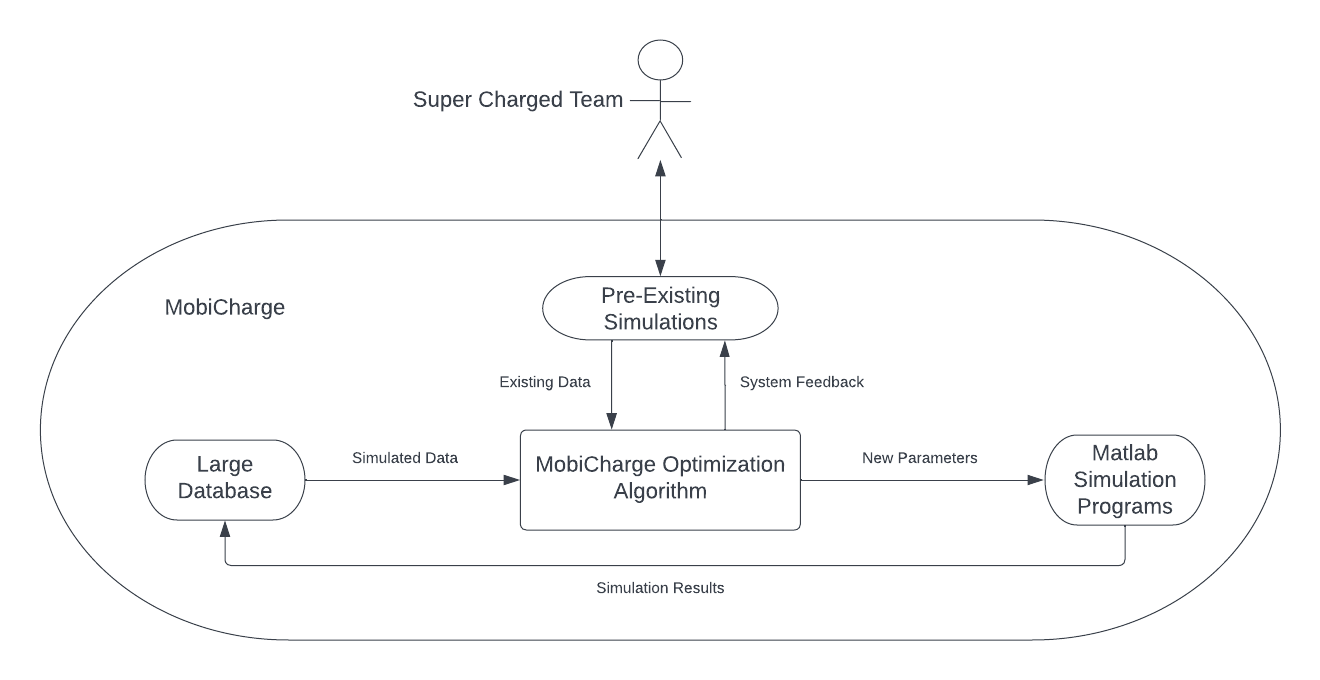
\includegraphics[width=15cm]{images/context1.png}
    \caption[Prelim System Contexts 2]{Second stage of the preliminary system context.}
    \label{fig:figure2}
\end{figure}
As shown in figure 2, the external entity, the Super Charged team, will then integrate the optimization algorithm with pre-existing simulation software. This will allow the system to conduct simulations automatically, furthering the knowledge base of the system
\newpage
\begin{figure}[htp]
    \centering
    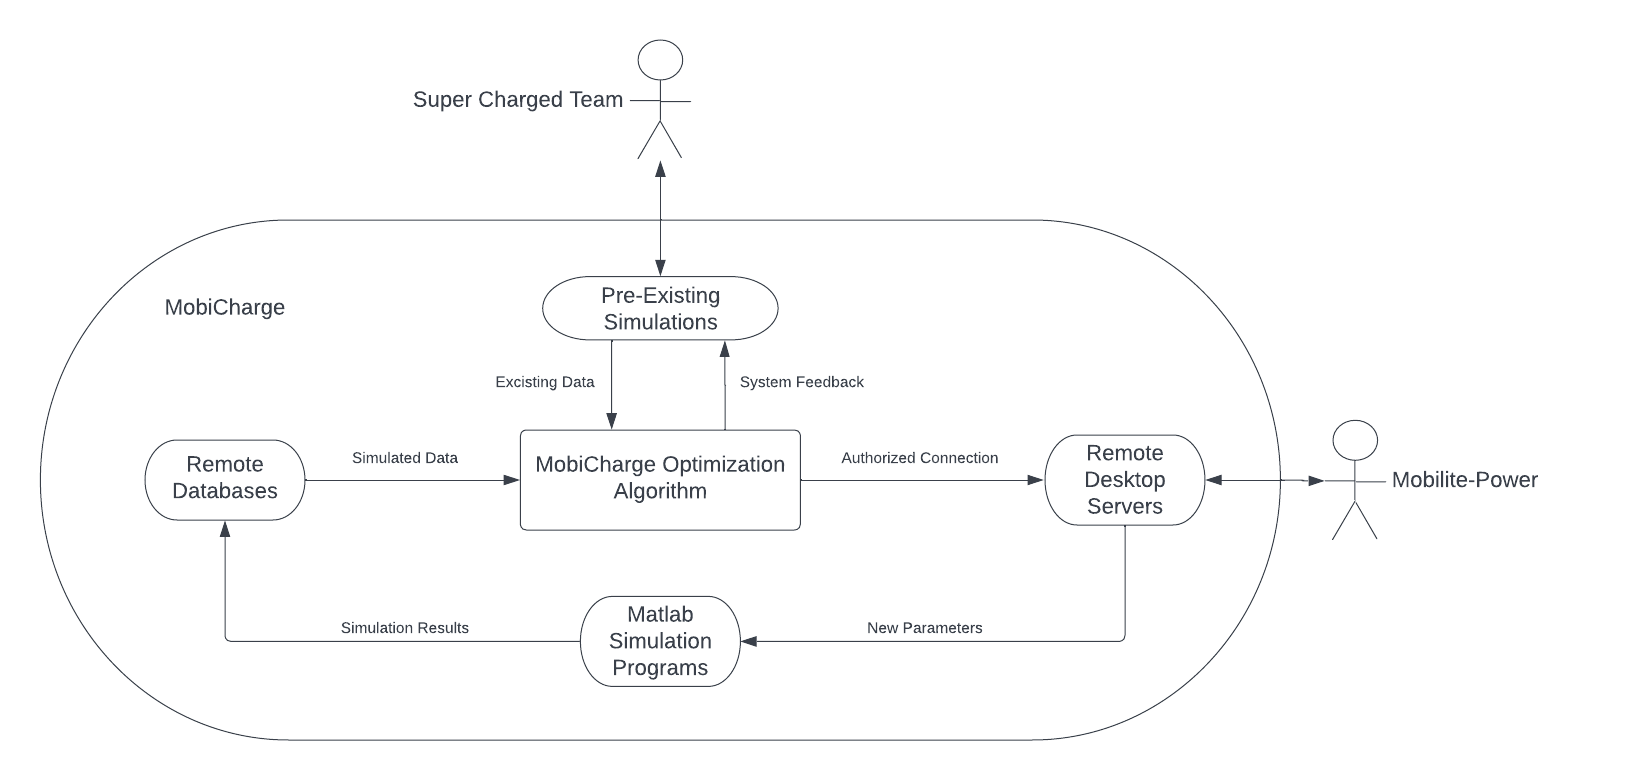
\includegraphics[width=15cm]{images/context2.png}
    \caption[Prelim System Contexts 3]{Final stage of the preliminary system context.}
    \label{fig:figure3}
\end{figure}
The last stage of the preliminary system context is as shown in figure 3. The external entities are the Super Charged team, as well as the MobilitePower company. Mobilite-Power is the external entity which oversees the data acquired from the simulations and provides clients with the necessary configurations for the remote charging devices. Mobilite-Power will provide access to remote desktop servers, which the Super Charged team will integrate into the system, allowing for more simulations to be accessed by the system. This will further train the system, increasing the accuracy of the optimizations produced by the system.

\newpage
\subsection{Server Integrated System Context}

\begin{figure}[htp]
    \centering
    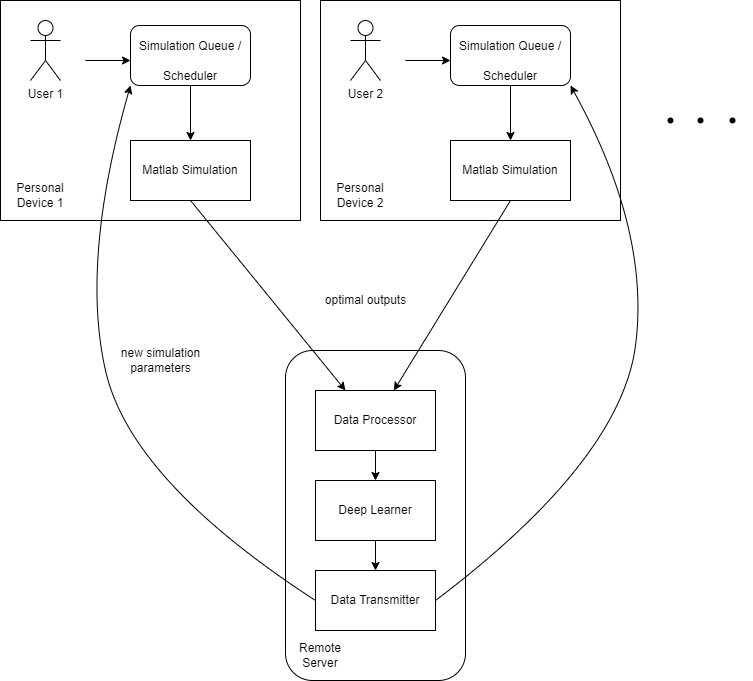
\includegraphics[width=15cm]{images/server_system.png}
    \caption[Server-Int System Contexts 1]{System context integrated with servers.}
    \label{fig:figure4}
\end{figure}

The divide between personal devices and the server will likely be structured as shown above, where the deep learner exists as a part of a central server, and the core computations of the simulations can be done on local machines. This allows the server to remain relatively low fidelity for the time being, where its core computations are the algorithms of the deep learner itself. The data processor and transmitters will handle concurrency and syncing with local devices. This obviously requires cooperation and coordination of these local devices, and this may not be ideal for commercial use. The goal is to prioritize data throughput in the development stage, leaving the simulations relatively untouched and implementing enough modularity such that the server can be formalized and protected with more elegance down the line, and integrated with higher-fidelity computing devices.

\subsection{Deployed System Context}
Once the system has been sufficiently trained and developed, it will be deployed for commercial use. However, the software system will continuously be trained and the throughput will continue to be refined. In a commercial setting, the system will interact with Mobilite-Power, who will feed the desired output to the system, and the system will produce the optimal configuration for a remote charging device. This data will be exported to the Mobilite-Power production team once the system has encrypted the data. The system will also be able to decrypt the data following the export and retrain the system with the optimized results. Lastly, the optimized data will be stored in a database to repeatedly enhance the accuracy of the system.
\newpage
\begin{figure}[htp]
    \centering
    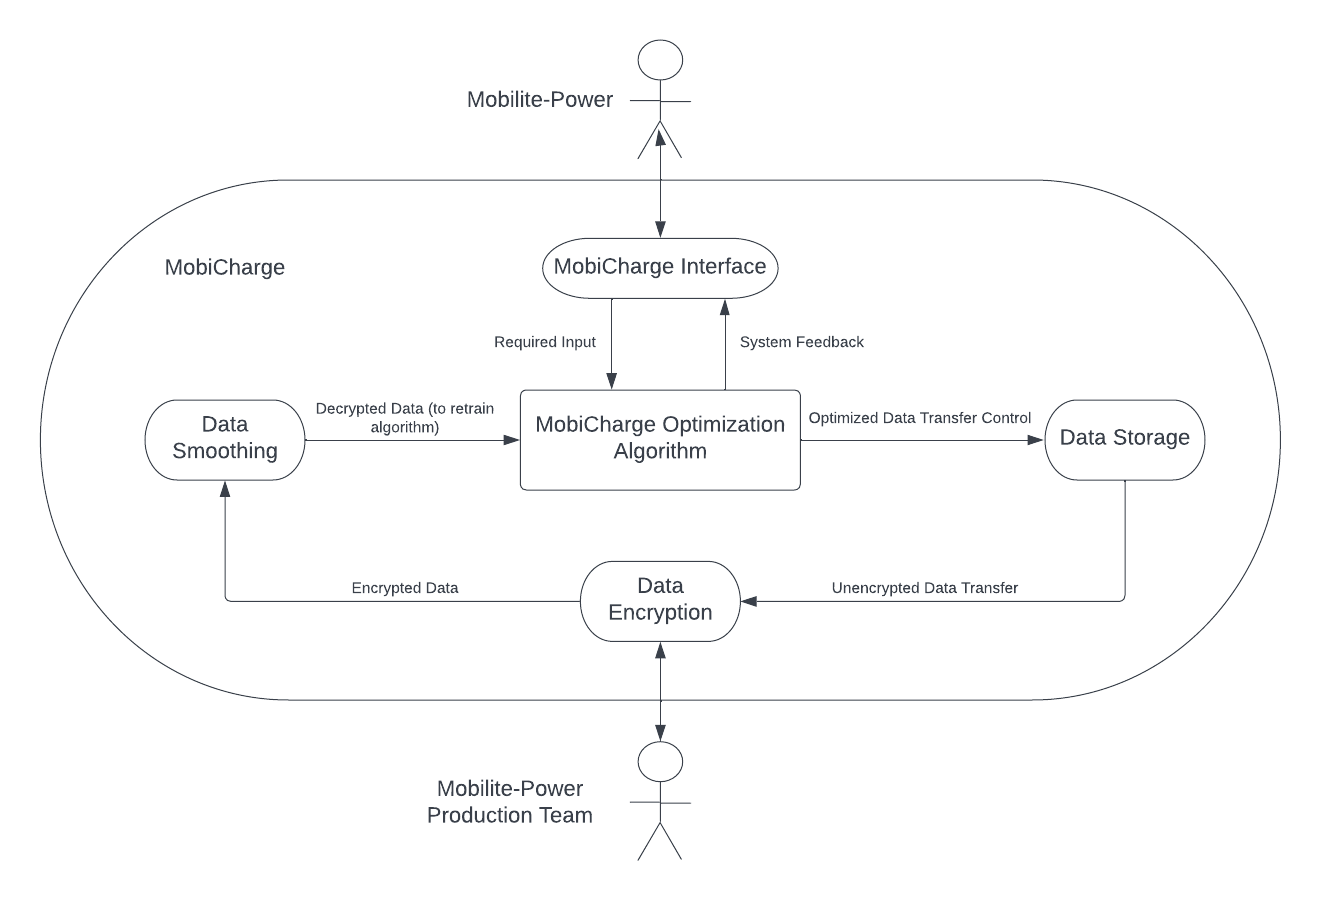
\includegraphics[width=15cm]{images/context3.png}
    \caption[Deployed System Contexts 1]{Stage of the deployed system context.}
    \label{fig:figure5}
\end{figure}
As shown in figure 5, the external entities acting on the system are the Mobilite-Power group responsible for determining the optimal configuration for the remote charging device, and the Mobilite-Power production team responsible for building the remote charging device. The Mobilite-Power entity will access the system and provide the desired output of the remote charging device. The system will then produce the optimal configuration and provide that configuration to the production team in an encrypted manner. 

\subsection{Hardware System Context}
The hardware system will be used by the MobiCharged team to validate parameters and be displayed for demonstration purposes. Due to limitations revolving around cost \& time constraints, the MobiCharged team proceeded with designing a system that simulates a remote charging device using an array of transducers connected to the system to levitate particles which will simulate remote charging devices, i.e. sending electromagnetic waves to the receiving ends of sensors. 

\begin{figure}[htp]
  \centering
  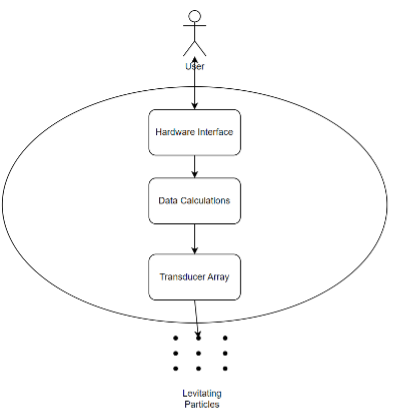
\includegraphics[width=7cm]{images/HardwareContext.png}
  \caption[Hardware Context]{Hardware System Context}
  \label{fig:figure6}
\end{figure}

As shown in Figure 6, the user can interact with the hardware interface to input data (such as desired location). The interface then sends those data points to the data calculations module in which the outputs (such as wavelength and phase) are calculated and then sent to the transducer array. Each transducer within the array will receive individual data such that the whole array can send constructive interfered waves to localized points. The particles will levitate due to the waves and can also move to other localized areas if intended to do so by the user. 

\subsection{Hardware System Parts}

Table 1 below lists the parts required to create the simulation for the physical remote charging devices. 

\begin{table}[H]
  \caption{\bf Parts List for Physical Remote Charging Simulation Device}
  \begin{tabular}{ |p{4cm}|p{3cm}|p{7cm}|} 
   \hline
  \bf Part & \bf Quantity\\
   \hline
   PCB: 183x169mm 2 layers & 1\\
   \hline
   MSO-P1040H07T Ultrasonic Emitter (Transducers) & 256\\
   \hline 
   CoreEP4CE6 FPGA & 1\\
   \hline 
   Drivers MIC4127 SOIC8 & 128\\
   \hline 
   shift-registers 74hc595 SOIC16 & 32\\
   \hline 
   0.1uf capacitors 50v 0805 & 160\\
   \hline 
   Arduino Nano or an USB-to-UART adaptor & 1\\
   \hline 
   DC barrel connector & 1\\
   \hline 
   Header Connectors for the FPGA (2x22) (2.54 pitch) & 1\\
   \hline 
   Side connectors either pin or headers (2x4 and 2x2) (2.54 pitch) & 1\\

  \end{tabular}
  \end{table}

\section{System Boundary}
\subsection{Preliminary Set of Monitored \& Controlled Variables}
The following is a list of all monitored and controlled variables.
\begin{table}[htp]
\caption{\bf Monitored \& Controlled Variables}
    \begin{tabular}{|p{4cm}|p{3cm}|p{7cm}|}
         \hline
         \bf Name & \bf Type & \bf Physical Interpretation\\
         \hline
         Charging Device's Range & Monitored & Maximum reach of for device charging.\\
         \hline
         Device's Lower Allowed Charge & Monitored & Minimum level of charge allowed in device before charging is required.\\
         \hline
         Device's Upper Desired Charge & Monitored & Level of charge desired in drive to be charged.\\
         \hline
         Wireless Charging Control & Controlled & \\
         \hline
         Displayed Device Charge & Controlled & \\
         \hline
         Current Supply & Controlled & Value of current supplied to charging device.\\
         \hline
         Charging Device Frequency & Controlled & Frequency used by charging device.\\
         \hline
         Phase Shift & Controlled & Phase shift used by charging device.\\
         \hline
    \end{tabular}
\end{table}


\subsection{Environment Variables}
\begin{table}[H]
\caption{\bf Environment Variables}
\begin{tabular}{ |p{4cm}|p{3cm}|p{7cm}|} 
 \hline
\bf Name & \bf Type & \bf Physical Interpretation\\
 \hline
 Position of Device to be Charged & Environmental & Relative distance from device to be charged to charging device.\\
 \hline
 Density of Medium & Environmental & Density of medium which charging device must charge through.\\
\hline
\end{tabular}
\end{table}
 
\section{Anticipated and Unlikely Changes}

\section{Module Hierarchy}
\subsection{Software System Module Hierarchy}
For the machine learning algorithm to be effective, it is efficient for it to be modularized. Below is a list and diagram of the software system module hierarchy, where further information upon these modules are outlined in the Module Decomposition section.

\subsection{Modules}
\begin{itemize}
  \item Input Module
  \item Initializer Module
  \item Machine Learner Blackboard Indirection Layer
  \item Database Access Module 1
  \item Database Access Module 2
  \item User Interface Module
  \item Controller / Server Module
  \item “Client” Module
\end{itemize}

\subsection{Hardware MOdule Hierarchy}
Although the physical simulation component of this project is not connected to the software portion directly, the hardware system can still be modularized to exhibit the workings of the system.
\par 
Below is a high-level module hierarchy of the hardware system where further information on each module will be described in the Module Decomposition section.Please note that the “modules” here can be more thought of to be component sections.
\par

\begin{itemize}
  \item PCB Board Module (includes MOSFET drivers, shift registers,  capacitors \& transducers i.e. electrosonic emitters)
  \item FPGA Module
  \item Power Supply Module (includes connectors \& ports)
  \item FPGA Programmer \& Arduino Module
\end{itemize}

For further illustrations of the components of the hardware system, below are diagrams depicting the connection between components.
\par 

\begin{figure}[htp]
  \centering
  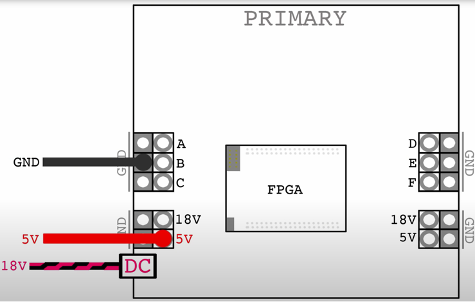
\includegraphics[width=7cm]{images/Figure8.png}
  \caption[PCB and Power]{PCB Board Component with FPGA \& Power Requirements}
  \label{fig:figure8}
\end{figure}

As shown in figure 8 above, the FPGA will be soldered onto the primary FPGA board for further ability of programming. The board will require a 5V power supply and a 9V power supply (note that the connector port is rated for 18V but 9V will be sufficient). 
\par 
Next we will connect the Arduino to the primary board as shown in figure 9 below.
\par

\begin{figure}[htp]
  \centering
  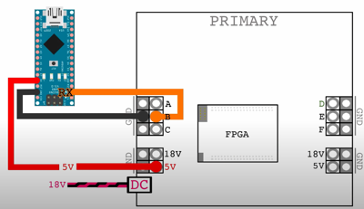
\includegraphics[width=7cm]{images/Figure9.png}
  \caption[Arduino Connectrion]{Arduino component connection to the PCB Board }
  \label{fig:figure9}
\end{figure}

In order to create a 3D levitation device for the purpose of simulating remote charging devices, a secondary board will be necessary. Figure 10 below shows the connections required.
\par 
\begin{figure}[htp]
  \centering
  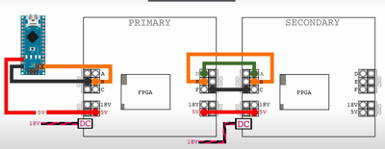
\includegraphics[width=7cm]{images/Figure10.png}
  \caption[Hardware Complete]{Complete 3D Levitation System}
  \label{fig:figure10}
\end{figure}

Note that for the whole system, the primary board \& secondary board will be on top of each other where the ultrasonic emitters (transducers) will be facing each other. There will be a sufficient gap in between the boards such that particles can be placed in between for levitation to occur and for it to be visible by the naked eye.
\par
Furthermore, the Arduino will be connected to the FPGA programmer component. In this case, it will be a PC running a Quartus software along with a script to operate the ultrasonic emitters.
\par
\section{Module Decomposition}
\subsection{Software Module Decomposition}
\begin{longtable}{|p{2cm}|p{3cm}|p{3cm}|p{3cm}}
  \caption{\bf Software Modules}\\
    \hline
    \bf Module & \bf Service & \bf Secret & \bf Estimated Completion\\
    \hline
    Initializer Module & Initializes main loop, and databases.  Allocates space for data processing, verifies that the MATLAB simulation compiles. Bounces errors if memory cannot be allocated or if MATLAB does not compile.  & The number of inputs/outputs that will determine how much memory is allocated, and the errors that can be returned. & End of January 2023. This module is finished for the most part. It may require slight edits when implementing with the other modules.\\
    \hline 
    Controller/ Server Module & Handles communication between the “Server” and “Client”. Passes inputs based on provided boundaries to Client module and returns optimal outputs. & The simulation inputs passed to client and the optimal outputs received by the client. & End of January 2023. This module is finished for the most part. It may require slight edits when implementing with the other modules.\\
    \hline 
    Client Module & Client module receives inputs and passes through MATLAB simulation and returns optimal outputs. & The MATLAB simulation format, simulation inputs and outputs. & End of January 2023. This module is finished for the most part. It may require slight edits when implementing with the other modules.\\
    \hline 
    Machine Learner Blackboard Indirection Layer & Reads batches of data from Database Access Module 1. Once certain data thresholds have been reached, this module passes batched data to specific model training streams. During downtimes where the amount of new data is received, this module will run validation test suites to monitor progress of models. Allows user requests for input into predictive models. This module will ultimately filter out the best performing models. & The data that is read from Database Access Module 1, format of validation tests, user requests, and trained models. & Feb-March. A large amount of simulation data still needs to be produced in order to train and test models.\\
    \hline 
    Database Access Module 1 & Stores the generated inputs and corresponding optimal output. Establishes basic reading and writing concurrency control. & The simulation inputs and optimal outputs that are stored in this database. & End of January 2023. This module is completed for the most part. However, the formatting of the database may require editing when simulation data is produced.\\
    \hline 
    Database Access Module 2 & Stores the generated hyperparameters and performance of each model stream in the Machine Learner Blackboard Indirection Layer. & The hyperparameters and model performances stored in this database. & Feb-March. A large amount of simulation data still needs to be produced in order to train and test models.\\
    \hline 
    User Interface Module & Controls the communication of the user prediction requests to the Machine Learner Blackboard Indirection Layer. It also displays the model performances after each validation test trial. & The results of the validation tests on the models, and the user requests. & Feb-March. This module requires the Machine Learner Blackboard Indirection Layer to be completed first. \\
    \hline 
\end{longtable}
  

\section{Traceablility Matrix}

\section{Use Hierarchy between Modules}

\section*{References}
We will be referring to documentations provided by Mobilite-Power, however, as of now there are no references to mention.

\bibliographystyle{plainnat}

\bibliography{SRS}

\newpage

\newpage{}
\section*{Appendix --- Reflection}

The information in this section will be used to evaluate the team members on the graduate attribute of Problem Analysis and Design. Please answer the following questions: 
\par 
\begin{enumerate}
  \item What are the limitations of your solution? Put another way, given unlimited resources, what could you do to make the project better? (LO ProbSolutions) 
  \item Give a brief overview of other design solutions you considered. What are the benefits and tradeoffs of those other designs compared with the chosen design? From all the potential options, why did you select documented design? (LO Explores)
\end{enumerate}

\begin{enumerate}  
  \item The limitations of our solution is primarily cost \& time. \par The problem of making the process of obtaining data values for the purpose of creating remote charging devices specific to certain applications easier is proposed to be solved through the methods of machine learning algorithms. That is, the process would become significantly easier if a machine learning algorithm could output the data values necessary at a much faster speed (and subsequently lower computational costs) without the use of simulations. \par The proposed solution has limitations in verifications. Through the original method of using simulations, the consequence is that it is extremely timely to output. However, the benefit of it is exhibited with verification of values. Through the machine learning algorithms, although the speed of the values being outputted increases significantly, the idea of verification becomes lost; particularly in the case where the algorithm goes past the limits of inputs provided. \par Given unlimited resources, the solution could become better if more time was present such that modules were created that verify the values and provide higher certainty in the values outputted. 
  Moreover, more servers would be purchased so that it may feed the machine learning algorithm without the use of users inputting data manually (referring to the client modules). \par 
  In regards to the hardware system, the proposed solution would become better with appropriate equipment to create a real prototype as opposed to a simulative one. The prototype would be better for display as well as feeding limits to the software by purchasing equipment such as antenna arrays, phase arrays, electromagnetic wave resistant encapsulations, etc. Moreover, with unlimited resources, the hardware system would be given an embedded system such that it may direct “charging” signals remotely to desired devices.
  \item An alternative solution for the design of this project was manually obtaining values based on certain inputs (and subsequently certain applications) over a wide range such that we may feed it into the machine learning algorithm. Although the benefit of this method is that the values are verified, it was better thought of to use a single server or two in order to run these simulations continuously in the backend automatically. This way, it is more efficient obtaining the values in the long term. In addition, this would be more effective for our client Mobilite Power as they can use the architecture of our software system and feed their large data set into it. This way, the machine learning algorithm will output more accurate results over a wider range of data. \par 
  Regarding the hardware system, an alternative solution was to create a small charging device using a pre-purchased antenna array. This would be done without the phase arrays but be implemented with a larger structure around the system to solve our stretch goals (which include being resistant to weather conditions). The benefit in this is that we can display different antenna array shapes \& sizing while illustrating the change in results; which we predicted to be power distributed as well as accuracy of electromagnetic waves sent. The problem with this solution is the limitation of resources. The group proceeded with creating a simulation of a remote charging device using a phased array system with the fear that the original solution mentioned would not be completed in a timely manner due to the expertise required. The original solution would dive into the area of PHD level projects and would be a risk in completion.   

\end{enumerate}


\end{document}

